% Copyright 2026  Ed Bueler

\documentclass[10pt,
               svgnames,
               hyperref={colorlinks,
                         citecolor=DeepPink4,
                         linkcolor=FireBrick,
                         urlcolor=blue},
               usepdftitle=false]{beamer}

\usetheme{Madrid}
\usecolortheme{beaver}
\setbeamercovered{transparent}
\setbeamerfont{frametitle}{size=\large}
\setbeamercolor*{block title}{bg=red!10}
\setbeamercolor*{block body}{bg=red!5}

\usepackage[english]{babel}
\usepackage[latin1]{inputenc}
\usepackage{times}
\usepackage[T1]{fontenc}
% Or whatever. Note that the encoding and the font should match. If T1
% does not look nice, try deleting the line with the fontenc.

\usepackage{fancyvrb,empheq,bm,xspace,dsfont,esint}
\usepackage{minted}
\usepackage{tikz}
\usetikzlibrary{positioning,arrows.meta}

% If you wish to uncover everything in a step-wise fashion, uncomment
% the following command: 
%\beamerdefaultoverlayspecification{<+->}

\newcommand{\bb}{\mathbf{b}}
\newcommand{\bc}{\mathbf{c}}
\newcommand{\bbf}{\mathbf{f}}
\newcommand{\bl}{\bm{\ell}}
\newcommand{\bn}{\mathbf{n}}
\newcommand{\bq}{\mathbf{q}}
\newcommand{\br}{\mathbf{r}}
\newcommand{\bs}{\mathbf{s}}
\newcommand{\bx}{\mathbf{x}}
\newcommand{\by}{\mathbf{y}}
\newcommand{\bv}{\mathbf{v}}
\newcommand{\bu}{\mathbf{u}}
\newcommand{\bw}{\mathbf{w}}

\newcommand{\bE}{\mathbf{E}}
\newcommand{\bV}{\mathbf{V}}

\newcommand{\cB}{\mathcal{B}}
\newcommand{\cE}{\mathcal{E}}
\newcommand{\cM}{\mathcal{M}}
\newcommand{\cR}{\mathcal{R}}

\newcommand{\bzero}{\bm{0}}

\newcommand{\CC}{\mathbb{C}}
\newcommand{\NN}{\mathbb{N}}
\newcommand{\RR}{\mathbb{R}}
\newcommand{\ZZ}{\mathbb{Z}}

\newcommand{\one}{\mathds{1}}

\newcommand{\Div}{\nabla\cdot}
\newcommand{\grad}{\nabla}

\renewcommand{\Re}{\operatorname{Re}}
\renewcommand{\Im}{\operatorname{Im}}

\newcommand{\range}{\operatorname{range}}
\newcommand{\Span}{\operatorname{span}}

\newcommand{\Matlab}{\textsc{Matlab}\xspace}
\newcommand{\eps}{\epsilon}

\newcommand{\Lloc}{L_{\text{loc}}^1}

\newcommand{\ds}{\displaystyle}

\newcommand{\ip}[2]{\left<#1,#2\right>}
\newcommand{\iip}[2]{\langle\!\langle #1, #2 \rangle\!\rangle}

\newcommand{\twovect}[4]{\ensuremath{{#1}_{#2} =
                            \begin{bmatrix} #3 \\ #4 \end{bmatrix}}}

\newcommand{\rbullet}{{\color{FireBrick} \bullet}}

\newcommand*\circled[1]{\tikz[baseline=(char.base)]{
            \node[shape=circle,draw,inner sep=2pt] (char) {#1};}}

\newcommand{\textbook}{Saxe, \emph{Beginning Functional Analysis}}

\DefineVerbatimEnvironment{mVerb}{Verbatim}{numbersep=2mm,
frame=lines,framerule=0.1mm,framesep=2mm,xleftmargin=4mm,fontsize=\scriptsize}

\setbeamertemplate{enumerate items}[ball]
\setbeamercolor{item projected}{bg=blue!70!black, fg=white}
\setbeamerfont{item projected}{size=\small}  % \small is *bigger* than default

\newcommand{\itemnum}[1]{\setcounter{enumi}{#1}\usebeamertemplate{enumerate item}}



\title[Why the EFM works]{Why the finite element method works}

\subtitle{calculations for week 14}

\author{Ed Bueler}

\institute[]{UAF Math 617 Functional Analysis}

\date{Spring 2026}


\begin{document}
\beamertemplatenavigationsymbolsempty

\begin{frame}
  \maketitle
\end{frame}


\begin{frame}{Outline}
  \tableofcontents[hideallsubsections]
\end{frame}

\AtBeginSection[]
{% do not put toc here this time
}


\section{recall: Poisson problem and its finite element (FE) approximation}

\begin{frame}{recall: the Sobolev spaces $H^1(\Omega)$ and $H_0^1(\Omega)$}

\begin{definition}
    $$H^1(\Omega) = \left\{f\in L^2(\Omega) \,\Big|\, \begin{matrix} \text{the weak derivative } f' \text{ exists} \\ \text{and is in } L^2(\Omega)\end{matrix}\right\}$$
is a Hilbert space with inner product and norm:
	$$\ip{f}{g}_{H^1} = \int_\Omega f(x) g(x)\,dx + \int_\Omega \grad f(x)\cdot \grad g(x)\,dx, \qquad \|f\|_{H^1} = \sqrt{\ip{f}{f}_{H^1}}$$
\end{definition}

\begin{definition}
    $$H_0^1(\Omega) = \overline{C_c^1(\Omega)},$$
(closure is in $H^1$ norm, and $H_0^1(\Omega)$ is a closed subspace of $H^1(\Omega)$)
\end{definition}
\end{frame}


\begin{frame}{recall: the weak form of a Poisson problem}

\begin{block}{notation}
   $$V=H_0^1(\Omega)$$
\end{block}

\begin{block}{weak form of the Poisson equation (homogeneous Dirichlet)}
Suppose $f\in L^2(\Omega)$ is given.  Find $u\in V$ so that
    $$\int_\Omega \grad u \cdot \grad v\,dx = \int_\Omega f v\,dx \quad \text{ for all test functions } v\in V$$
\end{block}
\end{frame}


\begin{frame}{recall: the piecewise-linear finite element space}

\begin{itemize}
\item suppose $\Omega \subset \RR^2$ is a polygon
\item put a mesh $\mathcal{T}$ of triangles on $\Omega$
\item denote nodes $x_i$ and triangles $T_k$

\vspace{-15mm}

\hfill % blobmesh.tikz  -- triangulated mesh on a blob-shaped 2D domain
% 10 boundary nodes, 5 interior nodes, 18 triangles
% usage:  \input{figs/blobmesh.tikz}
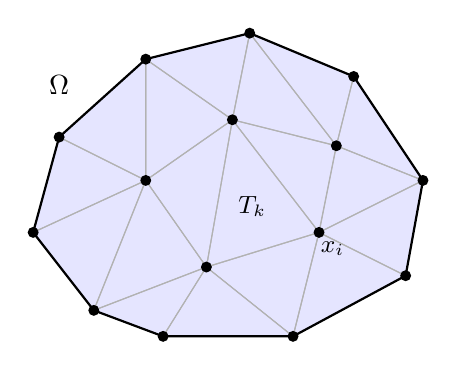
\begin{tikzpicture}[scale=1.1]

% boundary nodes
\coordinate (P0)  at ( 1.0,  0.0);
\coordinate (P1)  at ( 2.5,  0.0);
\coordinate (P2)  at ( 3.8,  0.7);
\coordinate (P3)  at ( 4.0,  1.8);
\coordinate (P4)  at ( 3.2,  3.0);
\coordinate (P5)  at ( 2.0,  3.5);
\coordinate (P6)  at ( 0.8,  3.2);
\coordinate (P7)  at (-0.2,  2.3);
\coordinate (P8)  at (-0.5,  1.2);
\coordinate (P9)  at ( 0.2,  0.3);

% interior nodes
\coordinate (P10) at ( 1.5,  0.8);
\coordinate (P11) at ( 2.8,  1.2);
\coordinate (P12) at ( 3.0,  2.2);
\coordinate (P13) at ( 1.8,  2.5);
\coordinate (P14) at ( 0.8,  1.8);

% filled triangles (light blue)
\fill[blue!10] (P9)  -- (P0)  -- (P10) -- cycle;
\fill[blue!10] (P0)  -- (P1)  -- (P10) -- cycle;
\fill[blue!10] (P1)  -- (P11) -- (P10) -- cycle;
\fill[blue!10] (P1)  -- (P2)  -- (P11) -- cycle;
\fill[blue!10] (P2)  -- (P3)  -- (P11) -- cycle;
\fill[blue!10] (P3)  -- (P12) -- (P11) -- cycle;
\fill[blue!10] (P3)  -- (P4)  -- (P12) -- cycle;
\fill[blue!10] (P4)  -- (P5)  -- (P12) -- cycle;
\fill[blue!10] (P5)  -- (P13) -- (P12) -- cycle;
\fill[blue!10] (P5)  -- (P6)  -- (P13) -- cycle;
\fill[blue!10] (P6)  -- (P14) -- (P13) -- cycle;
\fill[blue!10] (P6)  -- (P7)  -- (P14) -- cycle;
\fill[blue!10] (P7)  -- (P8)  -- (P14) -- cycle;
\fill[blue!10] (P8)  -- (P9)  -- (P14) -- cycle;
\fill[blue!10] (P9)  -- (P10) -- (P14) -- cycle;
\fill[blue!10] (P10) -- (P11) -- (P13) -- cycle;
\fill[blue!10] (P11) -- (P12) -- (P13) -- cycle;
\fill[blue!10] (P10) -- (P13) -- (P14) -- cycle;

% interior edges (gray, drawn before boundary)
\draw[gray!60, thin] (P9)  -- (P0)  -- (P10) -- cycle;
\draw[gray!60, thin] (P0)  -- (P1)  -- (P10) -- cycle;
\draw[gray!60, thin] (P1)  -- (P11) -- (P10) -- cycle;
\draw[gray!60, thin] (P1)  -- (P2)  -- (P11) -- cycle;
\draw[gray!60, thin] (P2)  -- (P3)  -- (P11) -- cycle;
\draw[gray!60, thin] (P3)  -- (P12) -- (P11) -- cycle;
\draw[gray!60, thin] (P3)  -- (P4)  -- (P12) -- cycle;
\draw[gray!60, thin] (P4)  -- (P5)  -- (P12) -- cycle;
\draw[gray!60, thin] (P5)  -- (P13) -- (P12) -- cycle;
\draw[gray!60, thin] (P5)  -- (P6)  -- (P13) -- cycle;
\draw[gray!60, thin] (P6)  -- (P14) -- (P13) -- cycle;
\draw[gray!60, thin] (P6)  -- (P7)  -- (P14) -- cycle;
\draw[gray!60, thin] (P7)  -- (P8)  -- (P14) -- cycle;
\draw[gray!60, thin] (P8)  -- (P9)  -- (P14) -- cycle;
\draw[gray!60, thin] (P9)  -- (P10) -- (P14) -- cycle;
\draw[gray!60, thin] (P10) -- (P11) -- (P13) -- cycle;
\draw[gray!60, thin] (P11) -- (P12) -- (P13) -- cycle;
\draw[gray!60, thin] (P10) -- (P13) -- (P14) -- cycle;

% boundary (thick, on top)
\draw[black, thick]
    (P0) -- (P1) -- (P2) -- (P3) -- (P4) -- (P5)
         -- (P6) -- (P7) -- (P8) -- (P9) -- cycle;

% nodes
\fill[black] (P0)  circle (1.8pt);
\fill[black] (P1)  circle (1.8pt);
\fill[black] (P2)  circle (1.8pt);
\fill[black] (P3)  circle (1.8pt);
\fill[black] (P4)  circle (1.8pt);
\fill[black] (P5)  circle (1.8pt);
\fill[black] (P6)  circle (1.8pt);
\fill[black] (P7)  circle (1.8pt);
\fill[black] (P8)  circle (1.8pt);
\fill[black] (P9)  circle (1.8pt);
\fill[black] (P10) circle (1.8pt);
\fill[black] (P11) circle (1.8pt);
\fill[black] (P12) circle (1.8pt);
\fill[black] (P13) circle (1.8pt);
\fill[black] (P14) circle (1.8pt);

% labels
\node[below right, font=\small, xshift=-1mm] at (P11) {$x_i$};
\node[font=\small] at (2.03, 1.5) {$T_k$};
\node at (-0.2, 2.9) {$\Omega$};

\end{tikzpicture}


\medskip
\item $f(x,y)=a + bx + cy$ is a \emph{linear polynomial} in two variables

\begin{definition}[the continuous $P_1$ finite element space over $\mathcal{T}$]
    $$P_1 = \left\{f \in C(\Omega)\,:\,f\big|_{T_k} \text{ is a linear polynomial}\right\}$$
\end{definition}

\item define the following \alert{finite-dimensional} subspace of $V$:
	$$V_h = \left\{f \in P_1\,:\,f\big|_{\partial\Omega} = 0\right\} \subset V=H_0^1(\Omega)$$
\end{itemize}
\end{frame}


\begin{frame}{recall the basic idea of the finite element method}

\begin{block}{weak form of the Poisson equation (homogeneous Dirichlet)}
Find $u\in V$ so that
    $$\int_\Omega \grad u \cdot \grad v\,dx = \int_\Omega f v\,dx \quad \forall v\in V$$
\end{block}

\begin{itemize}
\item FEM solves the \alert{same weak form}, but over a finite-dim'l subspace $V_h$
\end{itemize}

\begin{block}{an FEM for the Poisson equation (homogeneous Dirichlet)}
Find $u_h\in V_h$ so that
    $$\int_\Omega \grad u_h \cdot \grad v_h\,dx = \int_\Omega f v_h\,dx \quad \forall v_h\in V_h$$
\end{block}
\end{frame}


% at start of sections 2,3,... put outline
\AtBeginSection[] {
    \begin{frame}{Outline}
    \setbeamertemplate{section in toc}[sections numbered]
    \tableofcontents[currentsection]%,hideallsubsections]
    \end{frame}
}


\section{Cea's lemma: the FE approximation is the best}

\begin{frame}{xx}

\begin{itemize}
\item yy
\end{itemize}
\end{frame}


\section{examples}

\begin{frame}{xx}

\begin{itemize}
\item yy
\end{itemize}
\end{frame}


\section{interpolation}

\begin{frame}{xx}

\begin{itemize}
\item yy
\end{itemize}
\end{frame}


\section{convergence of the FE approximation}

\begin{frame}{xx}

\begin{itemize}
\item yy
\end{itemize}
\end{frame}


\section{lecture content in week 14}

\begin{frame}{lecture content in week 14}

\begin{itemize}
\item this material is only from slides
    \begin{itemize}
    \item[$\circ$] recalling the \href{https://bueler.github.io/fa/assets/slides/S26/week12.pdf}{week 12 slides} content is important
    \end{itemize}

\begin{block}{to know from these slides:}
\begin{itemize}
\item xx
\end{itemize}
\end{block}

%\item ?? Assignment 8 is posted at \quad  \href{https://bueler.github.io/fa/index.html}{\texttt{bueler.github.io/fa}}
\end{itemize}
\end{frame}

\end{document}
